\chapter{Ma trận và hệ phương trình tuyến tính}
\section{Ma trận}
\subsection{Định nghĩa và ký hiệu}
\subsubsection{Định nghĩa ma trận}
Một \textit{ma trận} $A$ cấp $m \times n$ trên $\mathbb{R}$ là một bảng chữ nhật gồm $m$ dòng $n$ cột mới $m \times n$ phần tử trong $\mathbb{R},$ có dạng
$$A = \left( {\begin{array}{*{20}{c}}
  {{a_{11}}}&{{a_{12}}}&{...}&{{a_{1n}}} \\ 
  {{a_{21}}}&{{a_{22}}}&{...}&{{a_{2n}}} \\ 
  {...}&{...}&{...}&{...} \\ 
  {{a_{m1}}}&{{a_{m2}}}&{...}&{{a_{mn}}} 
\end{array}} \right).$$
\subsubsection{Ký hiệu}
\begin{itemize}
\item $A = {\left( {{a_{ij}}} \right)_{m \times n}}$ hay $A = \left( {{a_{ij}}} \right),$ trong đó $a_{ij} \in \mathbb{R}.$ 
\item $a_{ij}$ hay $A_{ij}$ là phần tử ở vị trí dòng $i$ cột $j$ của $A.$
\item ${M_{m \times n}}\left( {\mathbb{R}} \right):$ tập hợp tất cả các ma trận cấp $m \times n$ trên $\mathbb{R}.$
\end{itemize}
\subsubsection{Ma trận không}
Ma trận cấp $m \times n$ có các phần tử đều bằng $0$ được gọi là \textit{ma trận không,} ký hiệu $0_{m \times n}$ (hay $0$).
\subsection{Ma trận vuông}
\subsubsection{Định nghĩa ma trận vuông}
\textit{Ma trận vuông} là ma trận có số dòng bằng số cột.
$$A = \left( {\begin{array}{*{20}{c}}
  {{a_{11}}}&{{a_{12}}}&{...}&{{a_{1n}}} \\ 
  {{a_{21}}}&{{a_{22}}}&{...}&{{a_{2n}}} \\ 
  {...}&{...}&{...}&{...} \\ 
  {{a_{n1}}}&{{a_{n2}}}&{...}&{{a_{nn}}} 
\end{array}} \right).$$
$M_n \left( {\mathbb{R}} \right):$ tập hợp tất cả các ma trận vuông cấp $n$ trên $\mathbb{R}.$
\subsubsection{Đường chéo chính}
Nếu $A = \left( {{a_{ij}}} \right) \in {M_n}\left( \mathbb{R} \right)$ thì đường chứa các phần tử $a_{11}, a_{22}, ..., a_{nn}$ được gọi là \textit{đường chéo chính} (hay \textit{đường chéo}) của $A.$
$$A = \left( {\begin{array}{*{20}{c}}
  {\mathbf{a_{11}}}&{{a_{12}}}&{...}&{{a_{1n}}} \\ 
  {{a_{21}}}&{\mathbf{a_{22}}}&{...}&{{a_{2n}}} \\ 
  {...}&{...}&{...}&{...} \\ 
  {{a_{n1}}}&{{a_{n2}}}&{...}&{\mathbf{a_{nn}}} 
\end{array}} \right).$$
\subsubsection{Ma trận tam giác, ma trận đường chéo}
Cho $A = \left( {a_{ij}} \right)$ là ma trận vuông. Khi đó
\begin{itemize}
\item Nếu các phần tử nằm dưới đường chéo của $A$ đều bằng $0$ (nghĩa là $a_{ij} = 0, \forall i > j$) thì $A$ được gọi là \textbf{\textit{ma trận tam giác trên.}}
\item Nếu các phần tử nằm trên đường chéo của $A$ đều bằng $0$ (nghĩa là $a_{ij} = 0, \forall i < j$) thì $A$ được gọi là \textbf{\textit{ma trận tam giác dưới.}}
\item Nếu mọi phần tử nằm ngoài đường chéo của $A$ đều bằng $0$ (nghĩa là $a_{ij} = 0, \forall i \ne j$) thì $A$ được gọi là \textbf{\textit{ma trận đường chéo,}} ký hiệu
$$A = \mathrm{diag}\left( {{a_1},{a_2},...,{a_n}} \right).$$
\end{itemize}
\begin{mybox}
\textbf{Nhận xét.} Ma trận $A$ là ma trận đường chéo khi và chỉ khi $A$ vừa là ma trận tam giác trên vừa là ma trận tam giác dưới.
\end{mybox}
\subsubsection{Ma trận đơn vị}
Ma trận vuông cấp $n$ có các phần tử trên đường chéo bằng $1,$ các phần tử nằm ngoài đường chéo bằng $0$ được gọi là \textit{ma trận đơn vị} cấp $n,$ ký hiệu $I_n$ (hoặc $I$).
\subsection{Các phép toán trên ma trận}
\subsubsection{So sánh hai ma trận}
Cho $A, B \in M_{m \times n} \left( {\mathbb{R}} \right).$ Khi đó, nếu $A_{ij} = B_{ij}, \forall i, j$ thì $A$ và $B$ được gọi là \textit{hai ma trận bằng nhau,} ký hiệu $A = B.$
\subsubsection{Chuyển vị ma trận}
Cho $A \in  M_{m \times n} \left( {\mathbb{R}} \right).$ Ta gọi \textit{ma trận chuyển vị} của $A,$ ký hiệu $A^\mathrm{T},$ là ma trận cấp $n \times m,$ có được từ $A$ bằng cách xếp các dòng của $A$ thành các cột tương ứng, nghĩa là
\begin{center}
$A = \left( {\begin{array}{*{20}{c}}
  {{a_{11}}}&{{a_{12}}}&{...}&{{a_{1n}}} \\ 
  {{a_{21}}}&{{a_{22}}}&{...}&{{a_{2n}}} \\ 
  {...}&{...}&{...}&{...} \\ 
  {{a_{m1}}}&{{a_{m2}}}&{...}&{{a_{mn}}} 
\end{array}} \right)$
 thì ${A^\mathrm{T}} = \left( {\begin{array}{*{20}{c}}
  {{a_{11}}}&{{a_{21}}}&{...}&{{a_{m1}}} \\ 
  {{a_{12}}}&{{a_{22}}}&{...}&{{a_{m2}}} \\ 
  {...}&{...}&{...}&{...} \\ 
  {{a_{1n}}}&{{a_{2n}}}&{...}&{{a_{mn}}} 
\end{array}} \right).$
\end{center}
\begin{mybox}
\textbf{Tính chất.}
Cho $A, B \in M_{m \times n} \left( {\mathbb{R}} \right).$ Khi đó:
\begin{itemize}
\item $\left( {A^{\mathrm{T}} }\right) ^ {\mathrm{T}} = A;$
\item $ A^{\mathrm{T}} = B ^ {\mathrm{T}} \Leftrightarrow A = B.$
\end{itemize}
\end{mybox}
\begin{mybox}
\textbf{Định nghĩa.} Cho $A$ là ma trận vuông. Nếu $A ^ {\mathrm{T}} = A$ thì ta nói $A$ là \textbf{\textit{ma trận đối xứng.}}
\end{mybox}
\subsubsection{Nhân một số với ma trận}
Cho ma trận $A \in M_{m \times n} \left( {\mathbb{R}} \right)$ và $\alpha \in \mathbb{R}.$ Ta định nghĩa \textit{tích} của $\alpha$ với $A$ (kí hiệu $\alpha A$) là ma trận được xác định bằng cách nhân các phần tử của $A$ với $\alpha,$ nghĩa là
$${\left( {\alpha A} \right)_{ij}}: = \alpha {A_{ij}},\forall i,j.$$
Nếu $\alpha = -1,$ ta ký  hiệu $\left( {-1} \right) A$ bởi $ -A$ và gọi là \textit{ma trận đối} của $A.$
\begin{mybox}
\textbf{Tính chất.} Cho $A$ là ma trận và $\alpha, \beta \in \mathbb{R},$ ta có
\begin{itemize}
\item $\left( {\alpha \beta} \right) A = \alpha \left( {\beta A} \right);$
\item $\left( {aA} \right) ^{\mathrm{T}} = \alpha A ^{\mathrm{T}};$
\item $0 \cdot A = 0$ và $1 \cdot A = A.$
\end{itemize}
\end{mybox}
\subsubsection{Tổng của hai ma trận}
Cho $A, B \in M_{m \times n} \left( {\mathbb{R}} \right).$ Khi đó \textit{tổng} của $A$ và $B,$ ký hiệu là $A + B,$ là ma trận được xác định bởi
$${\left( {A + B} \right)_{ij}}: = {A_{ij}} + {B_{ij}},\forall i,j.$$
\begin{mybox}
\textbf{Nhận xét.} Để tính $A + B$ thì:
\begin{itemize}
\item $A$ và $B$ cùng cấp;
\item Các vị trí tương ứng cộng lại.
\end{itemize}
\end{mybox}
\textbf{Ký hiệu.} $A - B := A + \left( {-B} \right)$ và được gọi là \textit{hiệu} của $A$ và $B.$ 
\begin{mybox}
\textbf{Tính chất.} Cho $A, B, C \in M_{m \times n} \left( {\mathbb{R}} \right)$ và $\alpha, \beta \in \mathbb{R},$ ta có
\begin{itemize}
\item $A + B = B + A$ (\textit{tính giao hoán});
\item $\left( {A + B} \right) + C = A + \left( {B + C} \right)$ (\textit{tính kết hợp});
\item $0 + A = A + 0 = A;$
\item $A + \left( { - A} \right) = \left( { - A} \right) + A = 0;$
\item ${\left( {A + B} \right)^{\mathrm{T}}} = {A^{\mathrm{T}}} + {B^{\mathrm{T}}};$
\item $\alpha \left( {A + B} \right) = \alpha A + \alpha B;$
\item $\left( {\alpha  + \beta } \right)A = \alpha A + \beta A;$
\item $\left( {\alpha  + \beta } \right)A = \alpha A + \beta A;$
\end{itemize}
\end{mybox}
\subsubsection{Tích của hai ma trận}
Cho hai ma trận $A \in M_{m \times n} \left( {\mathbb{R}} \right)$ và $B \in M_{n \times p} \left( {\mathbb{R}} \right).$ Khi đó, \textit{tích} của $A$ với $B$ (ký hiệu $AB$) là ma trận thuộc $M_{m \times p} \left( {\mathbb{R}} \right)$ được xác định bởi
$${\left( {AB} \right)_{ij}}: = \sum\limits_{k = 1}^n {{A_{ik}}{B_{kj}}} $$
$$\begin{array}{*{20}{c}}
  {\begin{array}{*{20}{c}}
  {}&{} 
\end{array}}&{ = {A_{i1}}{B_{1j}} + {A_{i2}}{B_{2j}} + ... + {A_{in}}{B_{nj}}.} 
\end{array}$$
\begin{figure}[H]
\begin{center}
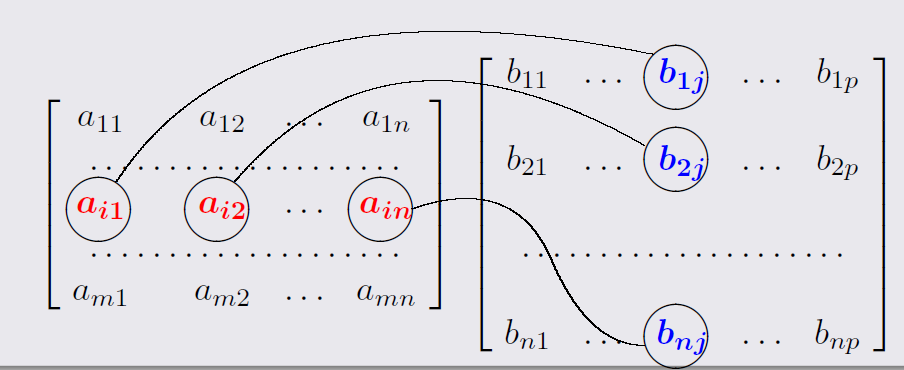
\includegraphics[scale=0.8]{C1_1}
\end{center}
\end{figure}
\begin{mybox}
\textbf{Nhận xét.} Để tính tích $AB$ thì
\begin{itemize}
\item Số cột của $A$ bằng số dòng của $B;$
\item Phần tử vị trí $i, j$ của $AB$ bằng dòng $i$ của $A$ nhân với cột $j$ của $B.$
\end{itemize}
\end{mybox}
\begin{mybox}
\textbf{Tính chất.} Cho $A \in {M_{m \times n}}\left( {\mathbb{R}} \right),B,{B_1},{B_2} \in {M_{n \times p}}\left( {\mathbb{R}} \right),C \in {M_{p \times q}}\left( {\mathbb{R}} \right),$ và ${D_1},{D_2} \in {M_{q \times m}}\left( {\mathbb{R}} \right).$ Khi đó
\begin{itemize}
\item ${I_m}A = A$ và $A{I_n} = A.$ Đặc biệt, với $A \in M_n \left( {\mathbb{R}} \right),$ ta có
$$ {I_n}A = A{I_n} = A.$$
\item $0_{p \times m}A = 0_{p \times n}$ và $A0_{n \times q} = 0_{m \times q}.$ Đặc biệt, với với $A \in M_n \left( {\mathbb{R}} \right),$ ta có
$$0_n A = A0_n = 0_n.$$
\item $\left( {AB} \right) ^{\mathrm{T}} = B ^{\mathrm{T}} A ^{\mathrm{T}}.$
\item $\left( {AB} \right) C  = A \left( {BC} \right).$
\item $A \left( {B_1 + B_2} \right) = AB_1 + AB_2.$
\item $ \left( {D_1 + D_2} \right) = D_1 A + D_2 A.$
\end{itemize}
\end{mybox}
\subsubsection{Lũy thừa ma trận}
Cho $A$ là ma trận vuông. Khi đó \textit{lũy thừa} bậc $k$ của $A,$ ký hiệu $A^k,$ được xác định như sau:
$${A^0}: = {I_n};{A^1}: = A;{A^2} = AA;...;{A^k} = {A^{k - 1}}A.$$
Như vậy ${A^k} = \underbrace {A...A}_{k \text{ lần}}.$
\begin{mybox}
\textbf{Tính chất.} Cho $A \in M_n \left( {\mathbb{R}} \right)$ và $k, l \in \mathbb{N}.$ Khi đó:
\begin{itemize}
\item $I_n^k = I_n;$
\item $A^k A^l = A^{k + l};$
\item $\left( {A^k} \right)^l = A^{kl}.$
\end{itemize}
\end{mybox}
\subsubsection{Đa thức ma trận}
Cho $A$ là ma trận vuông trêN $\mathbb{R}$ và
$$f\left( x \right) = {\alpha _m}{x^m} + {\alpha _{m - 1}}{x^{m - 1}} + ... + {\alpha _1}x + {\alpha _0}$$
là một đa thức biến $x$ trên $\mathbb{R}$ (nghĩa là ${\alpha _i} \in \mathbb{R},\forall i = \overline {0,m}$). Khi đó,
$$f\left( A \right): = {\alpha _m}{A^m} + {\alpha _{m - 1}}{A^{m - 1}} + ... + {\alpha _1}A + {\alpha _0}{I_n}$$
được gọi là \textit{đa thức theo ma trận $A.$}
\begin{mybox}
\textbf{Nhận xét.} Cho $A$ là ma trận vuông. Khi đó các hằng đẳng thức, nhị thức Newton vẫn đúng với $A.$
\end{mybox}
\section{Các phép biến đổi sơ cấp trên dòng}
\subsection{Các phép biến đổi sơ cấp trên dòng}
Cho $A \in M_{m \times n} \left( {\mathbb{R}} \right).$ Ta gọi \textit{phép biến đổi sơ cấp trên dòng,} viết tắt là BĐSCTD trên $A,$ là một trong ba loại biến đổi sau:
\begin{itemize}
\item \textbf{Loại 1.} Hoán vị hai dòng $i$ và $j$ $\left( {i \ne j} \right).$\\
\centerline{Ký hiệu: $d_i \leftrightarrow d_j$}
\item \textbf{Loại 2.} Nhân dòng $i$ với một số $\alpha \ne 0.$\\
\centerline{Ký hiệu: $\alpha d_i.$}
\item Cộng vào dòng $i$ với $\beta$ lần dòng $j$ $\left( {j \ne i} \right).$\\
\centerline{Ký hiệu: $d_i + \beta d_j$}
\end{itemize}
Với $\varphi$ là một phép biến đổi sơ cấp, ký hiệu $\varphi \left( A \right)$ là ma trận có được từ $A$ thông qua $\varphi.$
\begin{mybox}
\textbf{Nhận xét.} Với định nghĩa tương tự ta cũng có khái niệm các phép biến đổi sơ cấp trên cột: ${c_i} \leftrightarrow {c_j},\alpha {c_i},{c_i} + \beta {c_j}.$
\end{mybox}
\begin{mybox}
\textbf{Nhận xét.} Cho $A$ là ma trận và $\alpha \ne 0, \beta \in \mathbb{R}.$ Khi đó
\begin{itemize}
\item Nếu $\mathop  \to \limits^{{d_i} \leftrightarrow {d_j}} $ thì $A'\mathop  \to \limits^{{d_i} \leftrightarrow {d_j}} A;$
\item Nếu $A\mathop  \to \limits^{\alpha {d_i}} A'$ thì $A'\mathop  \to \limits^{\frac{1}{\alpha }{d_i}} A;$
\item Nếu $A\mathop  \to \limits^{{d_i} + \beta {d_j}} A'$ thì $A'\mathop  \to \limits^{{d_i} - \beta {d_j}} A.$
\end{itemize} 
\end{mybox}
\subsubsection{Tương đương dòng}
Cho $A, B \in M_{m \times n} \left( {\mathbb{R}} \right).$ Ta nói $A$ \textit{tương đương dòng} với $B,$ ký hiệu $A \sim B,$ nếu $B$ có được từ $A$ thông qua hữu hạn các phép biến đổi sơ cấp trên dòng nào đó. Vậy
\begin{center}
$A \sim B$ $\Leftrightarrow$ Tồn tại các phép BĐSCTD $\varphi_1, \varphi_2, ..., \varphi_k$ sao cho
$$A\mathop  \to \limits^{{\varphi _1}} {A_1}\mathop  \to \limits^{{\varphi _2}} ...\mathop  \to \limits^{{\varphi _k}}  = {A_k} = B.$$
\end{center}
\begin{mybox}
Quan hệ tương đương dòng của ma trận là một quan hệ tương đương, nghĩa là $\forall A, B, C \in M_{m \times n} \left( {\mathbb{R}} \right),$ ta có
\begin{itemize}
\item $A \sim A$ (tính phản xạ).
\item $A \sim B \Rightarrow B \sim A$ (tính đối xứng).
\item $A \sim B$ và $B \sim C$ $\Rightarrow A \sim C$ (tính bắc cầu).
\end{itemize}
\end{mybox}
\subsection{Ma trận bậc thang}
Cho $A \in M_{m \times n} \left( {\mathbb{R}} \right).$ Phần tử khác $0$ đầu tiên của một dòng kể từ bên trái qua được gọi là \textit{phần tử cơ sở} của dòng đó.\\
Một ma trận được gọi là \textit{ma trận bậc thang} nếu nó thỏa 2 tính chất sau:
\begin{itemize}
\item Các dòng bằng không (nếu có) luôn nằm dưới;
\item Phần tử cơ sở của dòng dưới luôn nằm bên phải so với phần tử cơ sở của dòng trên.
\end{itemize}
\subsubsection{Ma trận bậc thang rút gọn}
Ma trận $A$ được gọi là \textit{ma trận bậc thang rút gọn} nếu thỏa 3 điều kiện sau:
\begin{itemize}
\item $A$ là ma trận bậc thang.
\item Các phần tử cơ sở đều bằng $1.$
\item Trên cột có chứa phần tử cơ sở, các phần tử không phải phần tử cơ sở đều bằng $0.$
\end{itemize}
\subsection{Hạng của ma trận (dạng bậc thang)}
Nếu $A$ tương đương dòng với một ma trận bậc thang $B$ thì $B$ được gọi là một \textit{dạng bậc thang} của $A.$
\begin{mybox}
\textbf{Nhận xét.} Một ma trận $A$ thì có nhiều dạng bậc thang, tuy nhiên các dạng bậc thang của $A$ đều có số dòng khác không bằng nhau. Ta gọi số dòng khác không này là \textit{\textbf{hạng}} của $A$, ký hiệu $r \left( A \right).$
\end{mybox}
\begin{mybox}
Cho $A, B \in M_{m \times n} \left( {\mathbb{R}} \right).$ Khi đó:
\begin{itemize}
\item $0 \leqslant r \left( A \right) \leqslant \min \left\{ {m, n} \right\};$
\item $r \left( A \right) = 0 \Leftrightarrow A = 0;$
\item Nếu $A \sim B$ thì $r \left( A \right) = r \left( B \right);$
\item $r \left( {A^{\mathrm{T}}} \right) = r \left( A \right).$
\end{itemize}
\end{mybox}
Nếu $A$ tương đương dòng với một ma trận bậc thang rút gọn $B$ thì $B$ được gọi là \textit{dạng bậc thang rút gọn} của $A.$
\begin{mybox}
\begin{theorem}
Dạng bậc thang rút gọn của một ma trận $A $ là duy nhất, được ký hiệu là $R_A.$
\end{theorem}
\end{mybox}
\subsubsection{Thuật toán Gauss tìm một dạng bậc thang của $A = \left( a_{ij} \right) \in M_{m \times n} \left( {\mathbb{R}} \right)$}
\textbf{Bước 1.} Cho $i := 1, j := 1.$\\
\textbf{Bước 2.} Nếu $i > m$ hoặc $j > n$ thì kết thúc.\\
\textbf{Bước 3.}
\begin{itemize}
\item Nếu $a_{ij} \ne 0,$ thực hiện các phép biến đổi sau:\\
\centerline{${d_k} - \frac{{{a_{kj}}}}{{{a_{ij}}}}{d_i}$ với $k > i.$} \\
Sau đó $i := i + 1, j := j + 1$ và quay về bước 2.
\item Nếu $a_{ij} = 0$ thì sang bước 4.
\end{itemize}
\textbf{Bước 4.} 
\begin{itemize}
\item Nếu $a_{kj} \ne 0$ với một $k > i$ nào đó thì chọn một $k$ như vậy và thực hiện phép biến đổi $d_i \leftrightarrow d_k$ và quay về bước 3.
\item Nếu $a_{kj} = 0$ với mọi $k > i$ thì $j := j + 1$ và quay về bước 2.
\end{itemize}
\begin{mybox}
\textbf{Lưu ý.} Trong quá trình đưa về dạng bậc thang, ta nên sử dụng các phép biến đổi phù hợp để hạn chế việc tính toán các số không đẹp.
\end{mybox}
\begin{mybox}
\textbf{Lưu ý.} Vì $r \left( A \right) = r \left( {A^{\mathrm{T}}} \right)$ nên trong quá trình tính toán hạng của $A$ ta có thể sử dụng các \textit{phép biến đổi sơ cấp trên cột.}
\end{mybox}
\subsubsection{Thuật toán Gauss $-$ Jordan tìm dạng bậc thang rút gọn của $A = \left( a_{ij} \right) \in M_{m \times n} \left( {\mathbb{R}} \right)$}
Chỉ khác Thuật toán Gauss ở bước 3, ta cần thực hiện các phép biến đổi sau:
\begin{itemize}
\item $\frac{1}{a_{ij}} d_i.$
\item $d_k - a_{kj}d_i$ với mọi $k \ne i.$
\end{itemize}
\section{Hệ phương trình tuyến tính}
\subsection{Định nghĩa hệ phương trình tuyến tính}
Một \textit{hệ phương trình tuyến tính} trên $\mathbb{R}$ gồm $m$ phương trình, $n$ ẩn số là một hệ có dạng
\begin{equation}
\left\{ \begin{gathered}
  {a_{11}}{x_1} + {a_{12}}{x_2} + ... + {a_{1n}}{x_n} = {b_1}; \hfill \\
  {a_{21}}{x_1} + {a_{22}}{x_2} + ... + {a_{2n}}{x_n} = {b_2}; \hfill \\
  .............................................. \hfill \\
  {a_{m1}}{x_1} + {a_{m2}}{x_2} + ... + {a_{mn}}{x_n} = {b_m}, \hfill \\ 
\end{gathered}  \right.
\label{eq11}
\end{equation}
trong đó
\begin{itemize}
\item $a_{ij} \in \mathbb{R}:$ các hệ số;
\item $b_i \in \mathbb{R}:$ các hệ số tự do;
\item $x_1, x_2, ..., x_n:$ các ẩn số nhận giá trị trong $\mathbb{R}.$
\end{itemize}
Nếu (\ref{eq11}) có các hệ số tự do bằng $0$ thì ta nói (\ref{eq11}) là \textit{hệ phương trình tuyến tính thuần nhất} trên $\mathbb{R}.$\\
Đặt $$A = \left( {\begin{array}{*{20}{c}}
  {{a_{11}}}&{{a_{12}}}&{...}&{{a_{1n}}} \\ 
  {{a_{21}}}&{{a_{22}}}&{...}&{{a_{2n}}} \\ 
  {...}&{...}&{...}&{...} \\ 
  {{a_{m1}}}&{{a_{m2}}}&{...}&{{a_{mn}}} 
\end{array}} \right),\begin{array}{*{20}{c}}
  {}&{X = \left( {\begin{array}{*{20}{c}}
  {{x_1}} \\ 
  {{x_2}} \\ 
  {...} \\ 
  {{x_n}} 
\end{array}} \right)} 
\end{array},\begin{array}{*{20}{c}}
  {}&{B = } 
\end{array}\left( {\begin{array}{*{20}{c}}
  {{b_1}} \\ 
  {{b_2}} \\ 
  {...} \\ 
  {{b_n}} 
\end{array}} \right).$$
Ta gọi $A$ là \textit{ma trận hệ số,} $X$ là cột các \textit{ẩn,} $B$ là cột các \textit{hệ số tự do} của hệ (\ref{eq11}). Khi đó hệ (\ref{eq11}) được viết dưới dạng $AX = B.$\\
Ta gọi $\mathop A\limits^ \sim   = \left( {\left. A \right|B} \right)$ là \textit{ma trận mở rộng} (hay ma trận bổ sung) của hệ (\ref{eq11}).
\subsection{Nghiệm của hệ phương trình tuyến tính}
Ta nói $u = \left( {\alpha_1}, {\alpha_2}, ..., {\alpha_n} \right)$ là \textit{nghiệm} của hệ phương trình (\ref{eq11}) nếu ta thế $x_1 = \alpha_1, x_2 = \alpha_2, ..., x_n = \alpha_n$ thì tất cả các phương trình trong (\ref{eq11}) đều thỏa.\\
Hai hệ phương trình được gọi là \textit{tương đương} nhau nếu chúng có cùng tập nghiệm.
\begin{mybox}
\textbf{Nhận xét.} Khi giải một hệ phương trình tuyến tính, các phép biến đổi sau đây cho ta các hệ tương đương:
\begin{itemize}
\item Hoán đổi hai phương trình cho nhau.
\item Nhân hai vế của một phương trình với một số khác $0.$
\item Cộng vào một phương trình với một bội của phương trình khác.
\end{itemize}
\end{mybox}
\begin{mybox}
\begin{theorem}
Nếu hai hệ phương trình tuyến tính có ma trận mở rộng tương đương dòng với nhau thì hai hệ phương trình đó tương đương nhau.
\end{theorem}
\end{mybox}
\begin{mybox}
Nghiệm của hệ phương trình tuyến tính chỉ có 3 trường hợp sau:
\begin{itemize}
\item Vô nghiệm;
\item Duy nhất một nghiệm;
\item Vô số nghiệm.
\end{itemize}
\end{mybox}
\begin{mybox}
\textbf{Nhận xét.} Hệ phương trình tuyến tính thuần nhất
$$\left\{ \begin{gathered}
  {a_{11}}{x_1} + {a_{12}}{x_2} + ... + {a_{1n}}{x_n} = 0; \hfill \\
  {a_{21}}{x_1} + {a_{22}}{x_2} + ... + {a_{2n}}{x_n} = 0; \hfill \\
  ........................................... \hfill \\
  {a_{n1}}{x_1} + {a_{n2}}{x_2} + ... + {a_{nn}}{x_n} = 0, \hfill \\ 
\end{gathered}  \right.$$
luôn có một nghiệm $u = \left( {0, 0, ..., 0} \right).$ Nghiệm này được gọi là \textit{nghiệm tầm thường.}
\end{mybox}
\textbf{Lưu ý.} Đối với hệ phương trình tuyến tính thuần nhất, ta có các hệ số tự do bằng $0$ và không thay đổi khi ta thực hiện các phép biến đổi sơ cấp trên dòng. DO đó, khi giải hệ này ta chỉ cần sử dụng ma trận hệ số.
\subsection{Giải hệ phương trình tuyến tính}
Có 2 phương pháp giải hệ phương trình tuyến tính:
\begin{itemize}
\item Gauss: Đưa ma trận mở rộng về dạng bậc thang
\item Gauss $-$ Jordan: Đưa ma trận mở rộng về dạng bậc thang rút gọn.
\end{itemize}
\subsection{Định lí Kronecker $-$ Capelli}
\begin{mybox}
\begin{theorem}
Cho $\mathop A\limits^ \sim   = \left( {\left. A \right|B} \right)$ là ma trận mở rộng của hệ phương trình gồm $n$ ẩn $AX = B.$ Khi đó\\
\centerline{$r \left( {\mathop A\limits^ \sim} \right) = r \left( A \right)$ hoặc $r \left( {\mathop A\limits^ \sim} \right) = r \left( A \right) + 1.$}\\
Hơn nữa,
\begin{itemize}
\item nếu $r \left( {\mathop A\limits^ \sim} \right) = r \left( A \right) + 1$ thì hệ vô nghiệm;
\item nếu $r \left( {\mathop A\limits^ \sim} \right) = r \left( A \right) = n$ thì hệ có nghiệm duy nhất;
\item $r \left( {\mathop A\limits^ \sim} \right) = r \left( A \right) < n$ thì hệ có vô số nghiệm với bậc tự do là $ n - r \left( A \right).$
\end{itemize}
\end{theorem}
\end{mybox}
\section{Ma trận khả nghịch}
\subsection{Định nghĩa}
Cho $A \in M_n \left( {\mathbb{R}} \right).$ Ta nói $A$ \textit{khả nghịch} nếu tồn tại ma trận $B$ sao cho
$$AB = BA = I_n.$$
Nếu $B$ thỏa điều kiện trên được gọi là \textit{ma trận nghịch đảo} của $A.$\\
\textbf{Mệnh đề.} Ma trận nghịch đảo cảu một ma trận khả nghịch là duy nhất. Ta ký hiệu ma trận nghịch đảo của $A$ là $A^{-1}.$
\begin{mybox}
\begin{theorem}
Cho $A \in M_n \left( {\mathbb{R}} \right).$ Ma trận $A$ khả nghịch khi và chỉ khi tồn tại ma trận $B \in M_n \left( {\mathbb{R}} \right)$ sao cho $AB = I_n$ hay $BA = I_n.$ Khi đó $A^{-1} = B.$
\end{theorem}
\end{mybox}
\begin{mybox}
\textbf{Nhận xét.} 
\begin{itemize}
\item Ma trận đơn vị $I_n$ khả nghịch và $I_n^{-1} = I_n.$
\item Nếu $A \in M_n \left( {\mathbb{R}} \right)$ có một dòng hoặc một cột bằng không thì $A$ không khả nghịch.
\end{itemize}
\end{mybox}
\textbf{Mệnh đề.} Cho $A \in M_n \left( {\mathbb{R}} \right).$ Giả sử $A$ khả nghịch và có nghịch đảo là $A^{-1}.$ Khi đó
\begin{itemize}
\item $A^{-1}$ khả nghịch và $\left( {A^{-1}} \right)^{-1} = A.$
\item $A^{\mathrm{T}}$ khả nghịch và $\left( {A^{\mathrm{T}}} \right)^{-1} = \left( {A^{-1}} \right)^{\mathrm{T}}.$
\item $\forall \alpha \in \mathbb{R} \backslash \left\{ 0 \right\},$ $\alpha A$ khả nghịch và ${\left( {\alpha A} \right)^{ - 1}} = \frac{1}{\alpha }{A^{ - 1}}.$
\end{itemize}
\textbf{Mệnh đề.} Cho $A, B \in M_n \left( {\mathbb{R}} \right).$ Nếu $A$ và $B$ khả nghịch thì $AB$ cũng khả nghịch, hơn nữa
$${\left( {AB} \right)^{ - 1}} = {B^{ - 1}}{A^{ - 1}}.$$
\subsection{Nhận diện và tìm ma trận khả nghịch}
\begin{mybox}
\begin{theorem}
Cho $A \in M_n \left( {\mathbb{R}} \right).$ Khi đó các khẳng định sau tương đương:
\begin{itemize}
\item $A$ khả nghịch.
\item $r \left( A \right) = n.$
\item $A \sim I_n.$
\item Tồn tại các phép BĐSCTD $\varphi_1, \varphi_2, ..., \varphi_k$ biến ma trận $A$ thành ma trận đơn vị $I_n:$
$$A\mathop  \to \limits^{{\varphi _1}} {A_1}\mathop  \to \limits^{{\varphi _2}} ...\mathop  \to \limits^{{\varphi _k}}  = {A_k} = I_n.$$
Hơn nữa, khi đó qua chính các phép BĐSCTD $\varphi_1, \varphi_2, ..., \varphi_k,$ sẽ biến ma trận đơn vị $I_n$ thành ma trận nghịch đảo $A^{-1}:$
$$I_n\mathop  \to \limits^{{\varphi _1}} {B_1}\mathop  \to \limits^{{\varphi _2}} ...\mathop  \to \limits^{{\varphi _k}}  = {B_k} = A^{-1}.$$
\end{itemize}
\end{theorem}
\end{mybox}
\subsubsection{Phương pháp tìm ma trận nghịch đảo}
Lập $\left( {\left. A \right|{I_n}} \right)$ và dùng các phép BĐSCTD đưa $A$ về dạng ma trận bậc thang rút gọn:
$$\left( {\left. A \right|{I_n}} \right)\mathop  \to \limits^{{\varphi _1}} \left( {\left. {{A_1}} \right|{B_1}} \right) \to ...\mathop  \to \limits^{{\varphi _k}} \left( {\left. {{A_p}} \right|{B_p}} \right) \to ...$$
Trong quá trình biến đổi nếu xuất hiện ma trận $A_p$ có ít nhất một dòng hay một cột bằng không thì $A$ không khả nghịch.\\
Ngược lại ma trận cuối cùng của dãy trên có dạng $\left( {\left. {{I_n}} \right|B} \right).$ Khi đó $A$ khả nghịch và $A^{-1} = B.$\\
\textbf{Lưu ý.} Nếu bài toán chỉ yêu cầu kiểm tra ma trận $A$ có khả nghịch hay không thì ta chỉ cần tính hạng của ma trận (dùng thuật toán Gauss).
\section{Phương trình ma trận}
\begin{mybox}
\begin{theorem}
Cho các ma trận $A, A' \in M_n \left( {\mathbb{R}} \right)$ khả nghịch và $B \in {M_{n \times p}}\left( {\mathbb{R}} \right),C \in {M_{m \times n}}\left( {\mathbb{R}} \right),D \in {M_n}\left( {\mathbb{R}} \right).$
\begin{itemize}
\item $AX = B \Leftrightarrow X = {A^{-1}}B;$
\item $XA = C \Leftrightarrow X = C{A^{-1}};$
\item $AXA' = D \Leftrightarrow X = {A^{-1}}D{A'^{-1}}.$
\end{itemize}
\end{theorem}
\end{mybox}